\section{تمثيل الذراع باستخدام معاملات دينافيت-هارتنبرغ}

تُستخدم طريقة دينافيت-هارتنبرغ (\LR{Denavit-Hartenberg}) لوصف البنية الهندسية للذراع الروبوتية بصورة منهجية، وذلك من خلال تحديد مجموعة من الإطارات المرجعية المرتبطة بالمفاصل والوصلات. تتيح هذه الطريقة توصيف العلاقة بين كل وصلة والتي تليها باستخدام أربعة معاملات أساسية، مما يسهل اشتقاق الحركيات الأمامية للذراع الروبوتية.

في هذا الجزء، يتم تحديد الإطارات المرجعية لكل مفصل وفق قواعد \LR{DH}، ثم بناء جدول المعاملات الموافق للذراع الروبوتية ذات خمس درجات حرية المستخدمة في هذا المشروع.











\subsection{تحديد الإطارات المرجعية}

يتم تحديد الإطارات المرجعية في الأذرع الروبوتية اعتماداً على قواعد دينافيت–هارتنبرغ \LR{(Denavit--Hartenberg)}، والتي تُستخدم لوصف العلاقة الهندسية بين الوصلات المتتالية بطريقة منهجية.

بشكل عام، يتم تعريف المحاور وفق القواعد التالية:

\begin{itemize}
    \item يُعرَّف المحور \(z_i\) على أنه محور الحركة للمفصل \(i\)، أي محور الدوران في حالة المفاصل الدورانية أو محور الانزلاق في حالة المفاصل الخطية.
    \item يُختار المحور \(x_i\) بحيث يكون عمودياً على كل من \(z_{i-1}\) و\(z_i\)، أو على امتداد العمود المشترك بينهما في حال وجوده.
    \item يُحدد المحور \(y_i\) باستخدام قاعدة اليد اليمنى لضمان الحصول على جهاز إحداثي متعامد وموجب.
\end{itemize}

تسمح هذه القواعد بتعريف إطار مرجعي عند كل مفصل، مما يتيح استخراج معاملات دينافيت–هارتنبرغ وبناء مصفوفات التحويل المتجانس اللازمة لتحليل الحركة.

في هذا المشروع، تم تطبيق هذه القواعد على الذراع الروبوتية المدروسة، حيث تم تحديد الإطارات المرجعية لكل مفصل كما هو موضح في الشكل~\ref{fig:DH_frames}.
\begin{figure}[htbp]
\centering
\vspace*{\fill}
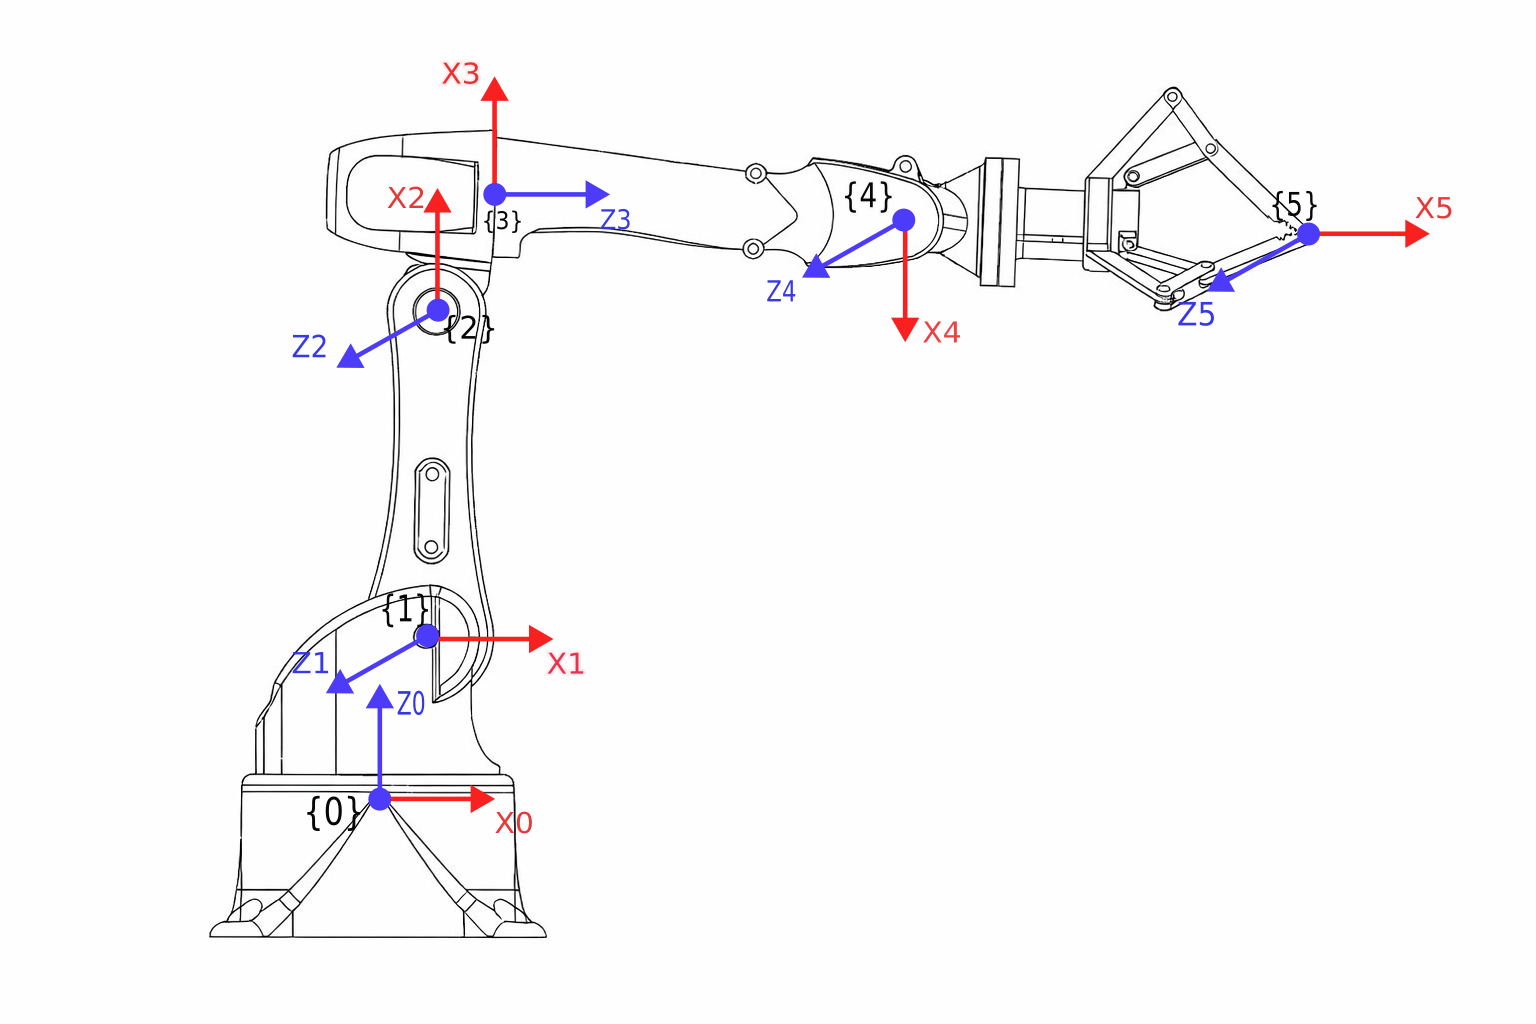
\includegraphics[width=0.8\textwidth]{resources/images/DHwith_Arm}
\captionof{figure}{\centering تحديد الإطارات المرجعية للذراع الروبوتية وفق قواعد دينافيت–هارتنبرغ}
\label{fig:DH_frames}
\vspace*{\fill}
\end{figure}
\clearpage

بناءً على تحديد الإطارات المرجعية، وبعد تعيين الأبعاد الهندسية للذراع الروبوتية كما هو مبين في الشكل~\ref{fig:frames}، يمكن استخراج معاملات دينافيت–هارتنبرغ التي تصف العلاقة بين الوصلات المتتالية.
\begin{figure}[htbp]
\centering
\vspace*{\fill}
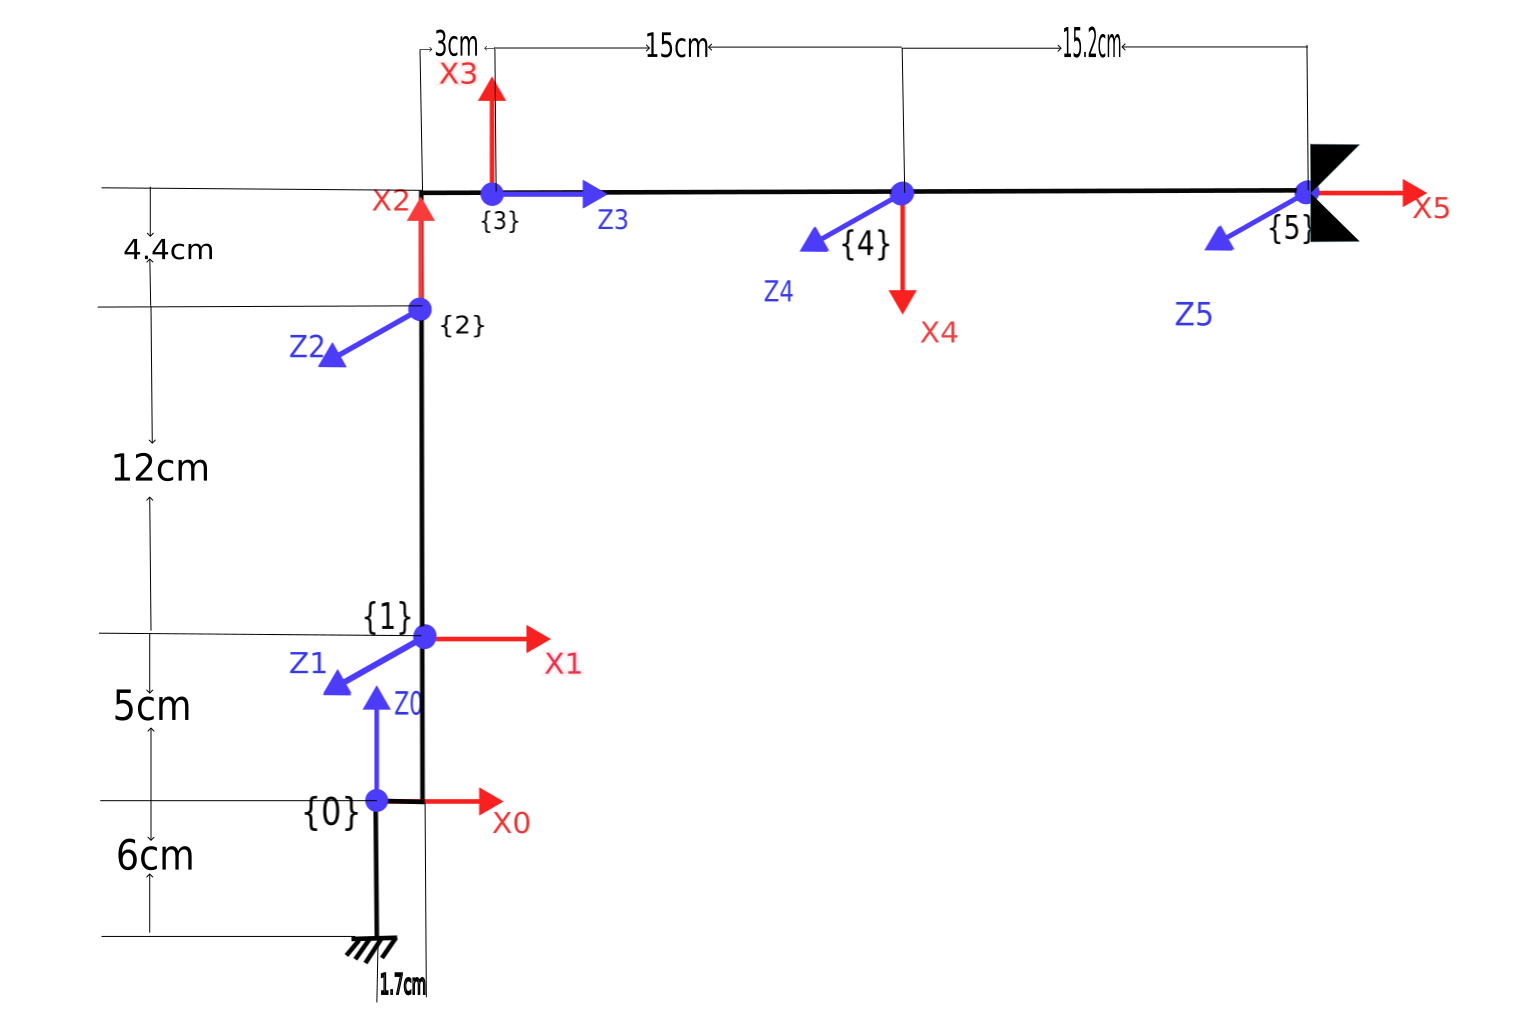
\includegraphics[width=0.8\textwidth]{resources/images/DH_frames}
\captionof{figure}{\centering تحديد الإطارات المرجعية للذراع الروبوتية وفق قواعد دينافيت–هارتنبرغ}
\label{fig:frames}
\vspace*{\fill}
\end{figure}

ومن خلال هذه القيم الهندسية واتجاهات المحاور، نجد أن جدول معاملات دينافيت–هارتنبرغ للذراع الروبوتية المدروسة يكون كما يلي:











\subsection{ جدول معاملات دينافيت–هارتنبرغ } 

يُستخدم تمثيل دينافيت–هارتنبرغ \LR{(Denavit–Hartenberg)} لوصف البنية الهندسية للذراع الروبوتية بطريقة منهجية، حيث يتم تحديد علاقة كل وصلة بالوصلة التي تسبقها باستخدام أربعة معاملات أساسية لكل مفصل.

لاستخراج معاملات DH، يتم أولاً تثبيت جهاز إحداثيات \LR{(Coordinate Frame)} لكل وصلة بحيث يكون المحور $z_i$ منطبقًا على محور دوران المفصل، بينما يُختار المحور $x_i$ عموديًا على كل من $z_i$ و $z_{i-1}$ أو على امتداد المسافة المشتركة بينهما.

بعد تحديد الأجهزة الإحداثية، يتم تعريف معاملات DH الأربعة كما يلي:

\begin{itemize}
\item $\theta_i$: زاوية الدوران حول المحور $z_{i-1}$، وتمثل المتغير المفصلي في حالة المفاصل الدورانية.
\item $d_i$: الإزاحة على طول المحور $z_{i-1}$.
\item $a_i$: طول الوصلة، وهو المسافة بين المحورين $z_{i-1}$ و $z_i$ على طول المحور $x_i$.
\item $\alpha_i$: زاوية الالتواء بين المحورين $z_{i-1}$ و $z_i$ حول المحور $x_i$.
\end{itemize}

بناءً على الأبعاد الهندسية للذراع الروبوتية المدروسة، يمكن تحديد هذه المعاملات لكل وصلة كما هو موضح في الجدول التالي:
\begin{table}[htbp]
%\begin{flushleft}
\centering
\resizebox{0.6\textwidth}{!}{

\begin{tabular}{|c|c|c|c|c|}
\hline
 $\theta_i$ & $d_i$ & $\alpha_i$ & $a_i$ &$i$ \\
\hline


$\theta_1$                   & $5cm$  & $90^\circ$  & $1.7cm$  &  1  \\
\hline
$\theta_2+90^\circ$          & $0cm$  & $0^\circ$   & $12cm$   &  2  \\
\hline
$\theta_3$                   & $0cm$  & $90^\circ$  & $4.4cm$  &  3  \\
\hline
$\theta_4+180^\circ$         & $15cm$ & $90^\circ$  & $0cm$    &  4  \\
\hline
$\theta_5+90^\circ$          & $0cm$  & $0^\circ$   & $15.2cm$ &  5  \\


\bottomrule

\end{tabular}
}
\captionof{figure}{\centering جدول معاملات دينافيت–هارتنبرغ}
\label{tab:DH}
%\end{flushleft}
\end{table}
